\chapter{Methodology}
\label{ch:methodology}

This chapter delineates the practical implementation of the theoretical cryptographic primitives discussed in Chapter \ref{ch:theory}. The methodology section details the concrete architecture of the password manager, explicitly defining how AES, HMAC, and PBKDF2 are orchestrated to construct a secure computational pipeline and a robust data storage format.

\section{Implementation Environment and Primitives}

To ensure complete control over the cryptographic lifecycle, the system is implemented using the \textbf{Python 3.11} ecosystem. The core cryptographic operations leverage the \textit{Hazardous Materials} (hazmat) layer of the \texttt{cryptography} library. This design choice is critical for academic transparency, as it requires the explicit management of low-level primitives—such as initialization vectors, padding schemes, and MAC composition—rather than relying on high-level, opaque abstractions like \texttt{Fernet}.

\begin{lstlisting}[language=Python, caption=Explicit Cryptographic Implementation Pipeline, label=lst:pipeline]
def derive_keys(password: str, salt: bytes, iterations: int):
    # PBKDF2 with SHA256 for Key Stretching
    kdf = PBKDF2HMAC(
        algorithm=hashes.SHA256(),
        length=32, salt=salt, iterations=iterations
    )
    full_key = kdf.derive(password.encode())
    # Key Splitting: 16b for AES + 16b for HMAC
    return full_key[:16], full_key[16:]

def encrypt_vault(data_bytes: bytes, aes_key: bytes, hmac_key: bytes):
    # 1. PKCS7 Padding for Block Alignment
    padder = padding.PKCS7(128).padder()
    padded_data = padder.update(data_bytes) + padder.finalize()

    # 2. Encryption: AES-128-CBC with CSPRNG IV
    iv = secrets.token_bytes(16)
    cipher = Cipher(algorithms.AES(aes_key), modes.CBC(iv))
    encryptor = cipher.encryptor()
    ciphertext = encryptor.update(padded_data) + encryptor.finalize()

    # 3. Integrity: HMAC-SHA256 (Encrypt-then-MAC)
    h = hmac.HMAC(hmac_key, hashes.SHA256())
    h.update(ciphertext)
    mac_tag = h.finalize()

    return iv, mac_tag, ciphertext
\end{lstlisting}

\section{Cryptographic Pipeline}

\subsection{System Flow Overview}
The core operational logic of the password manager is deterministically driven by the user's Master Password. Figure \ref{fig:enc_flow} illustrates the encryption pipeline, transitioning from the initial password to the final secure vault. The process initiates with PBKDF2 deriving a Master Key, which is subsequently split into independent keys for encryption and authentication. 

\begin{figure}[H]
    \centering
    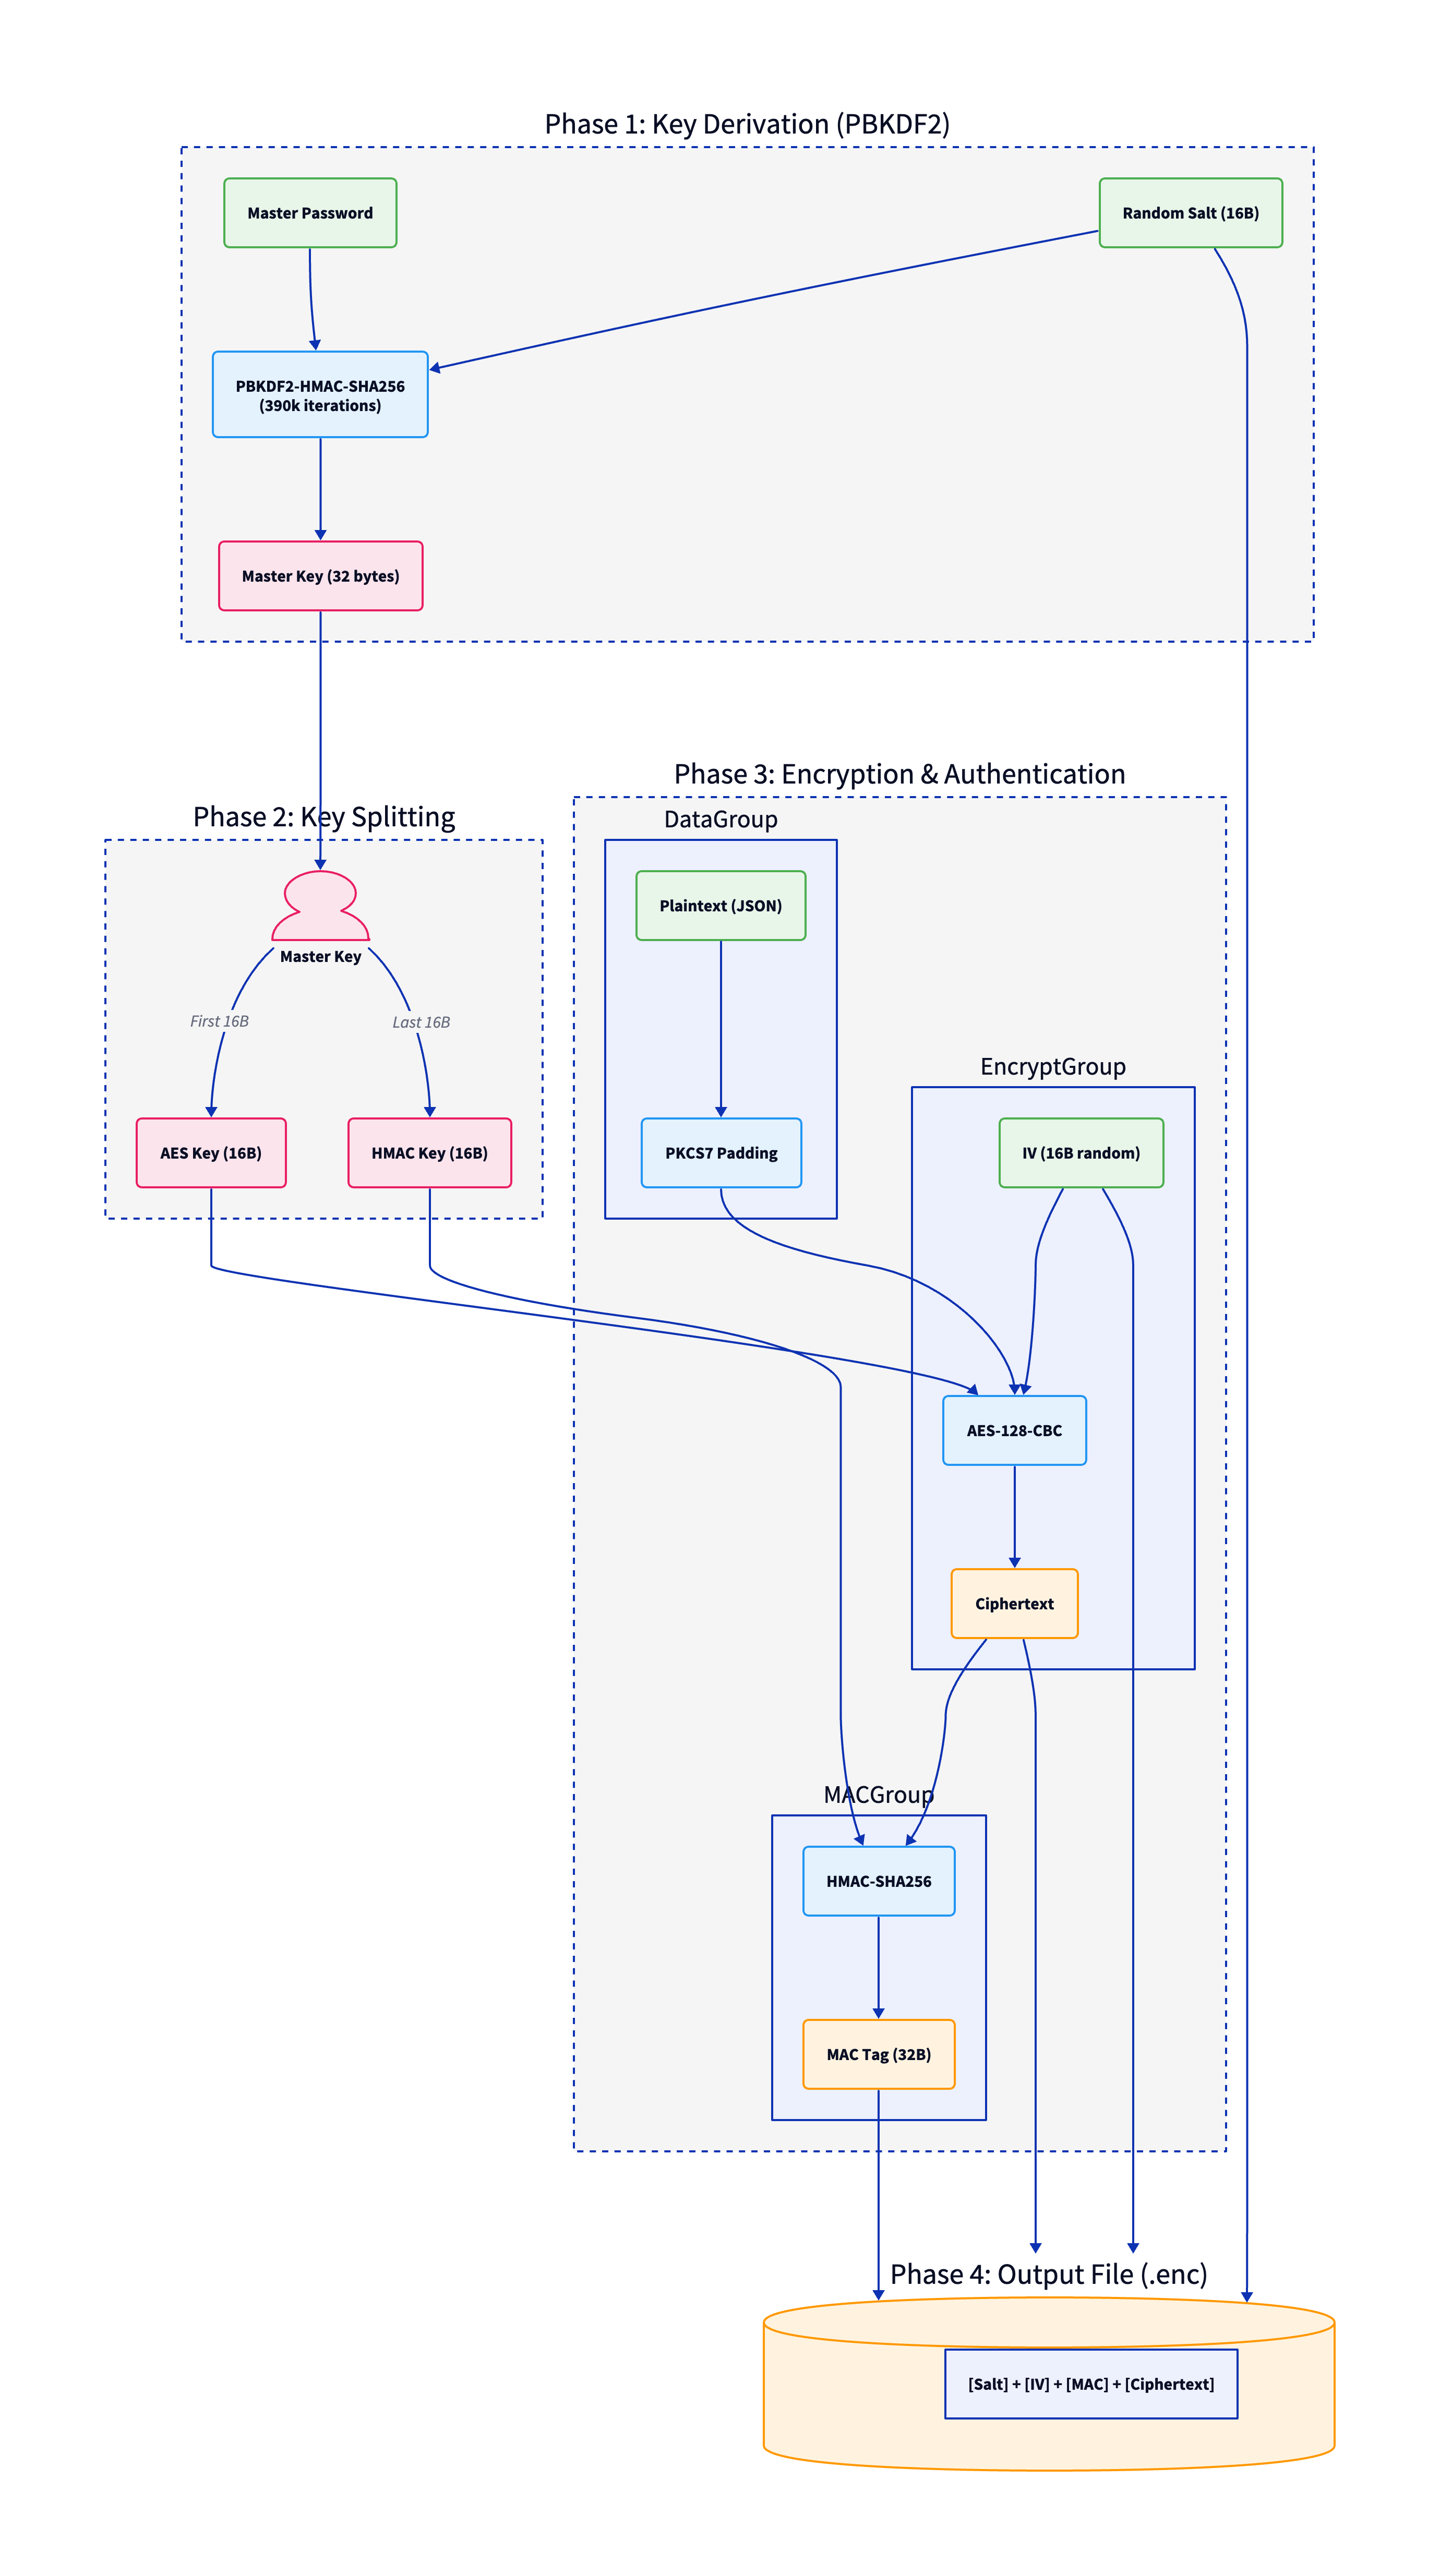
\includegraphics[width=0.8\textwidth]{../figure/figure_1a_encryption_flow.png}
    \caption{Phase-based Encryption Pipeline}
    \label{fig:enc_flow}
\end{figure}

Conversely, Figure \ref{fig:dec_flow} demonstrates the decryption pipeline. This routine rigidly enforces the security invariants established during encryption by verifying the authentication tag prior to any decryption attempt.

\begin{figure}[H]
    \centering
    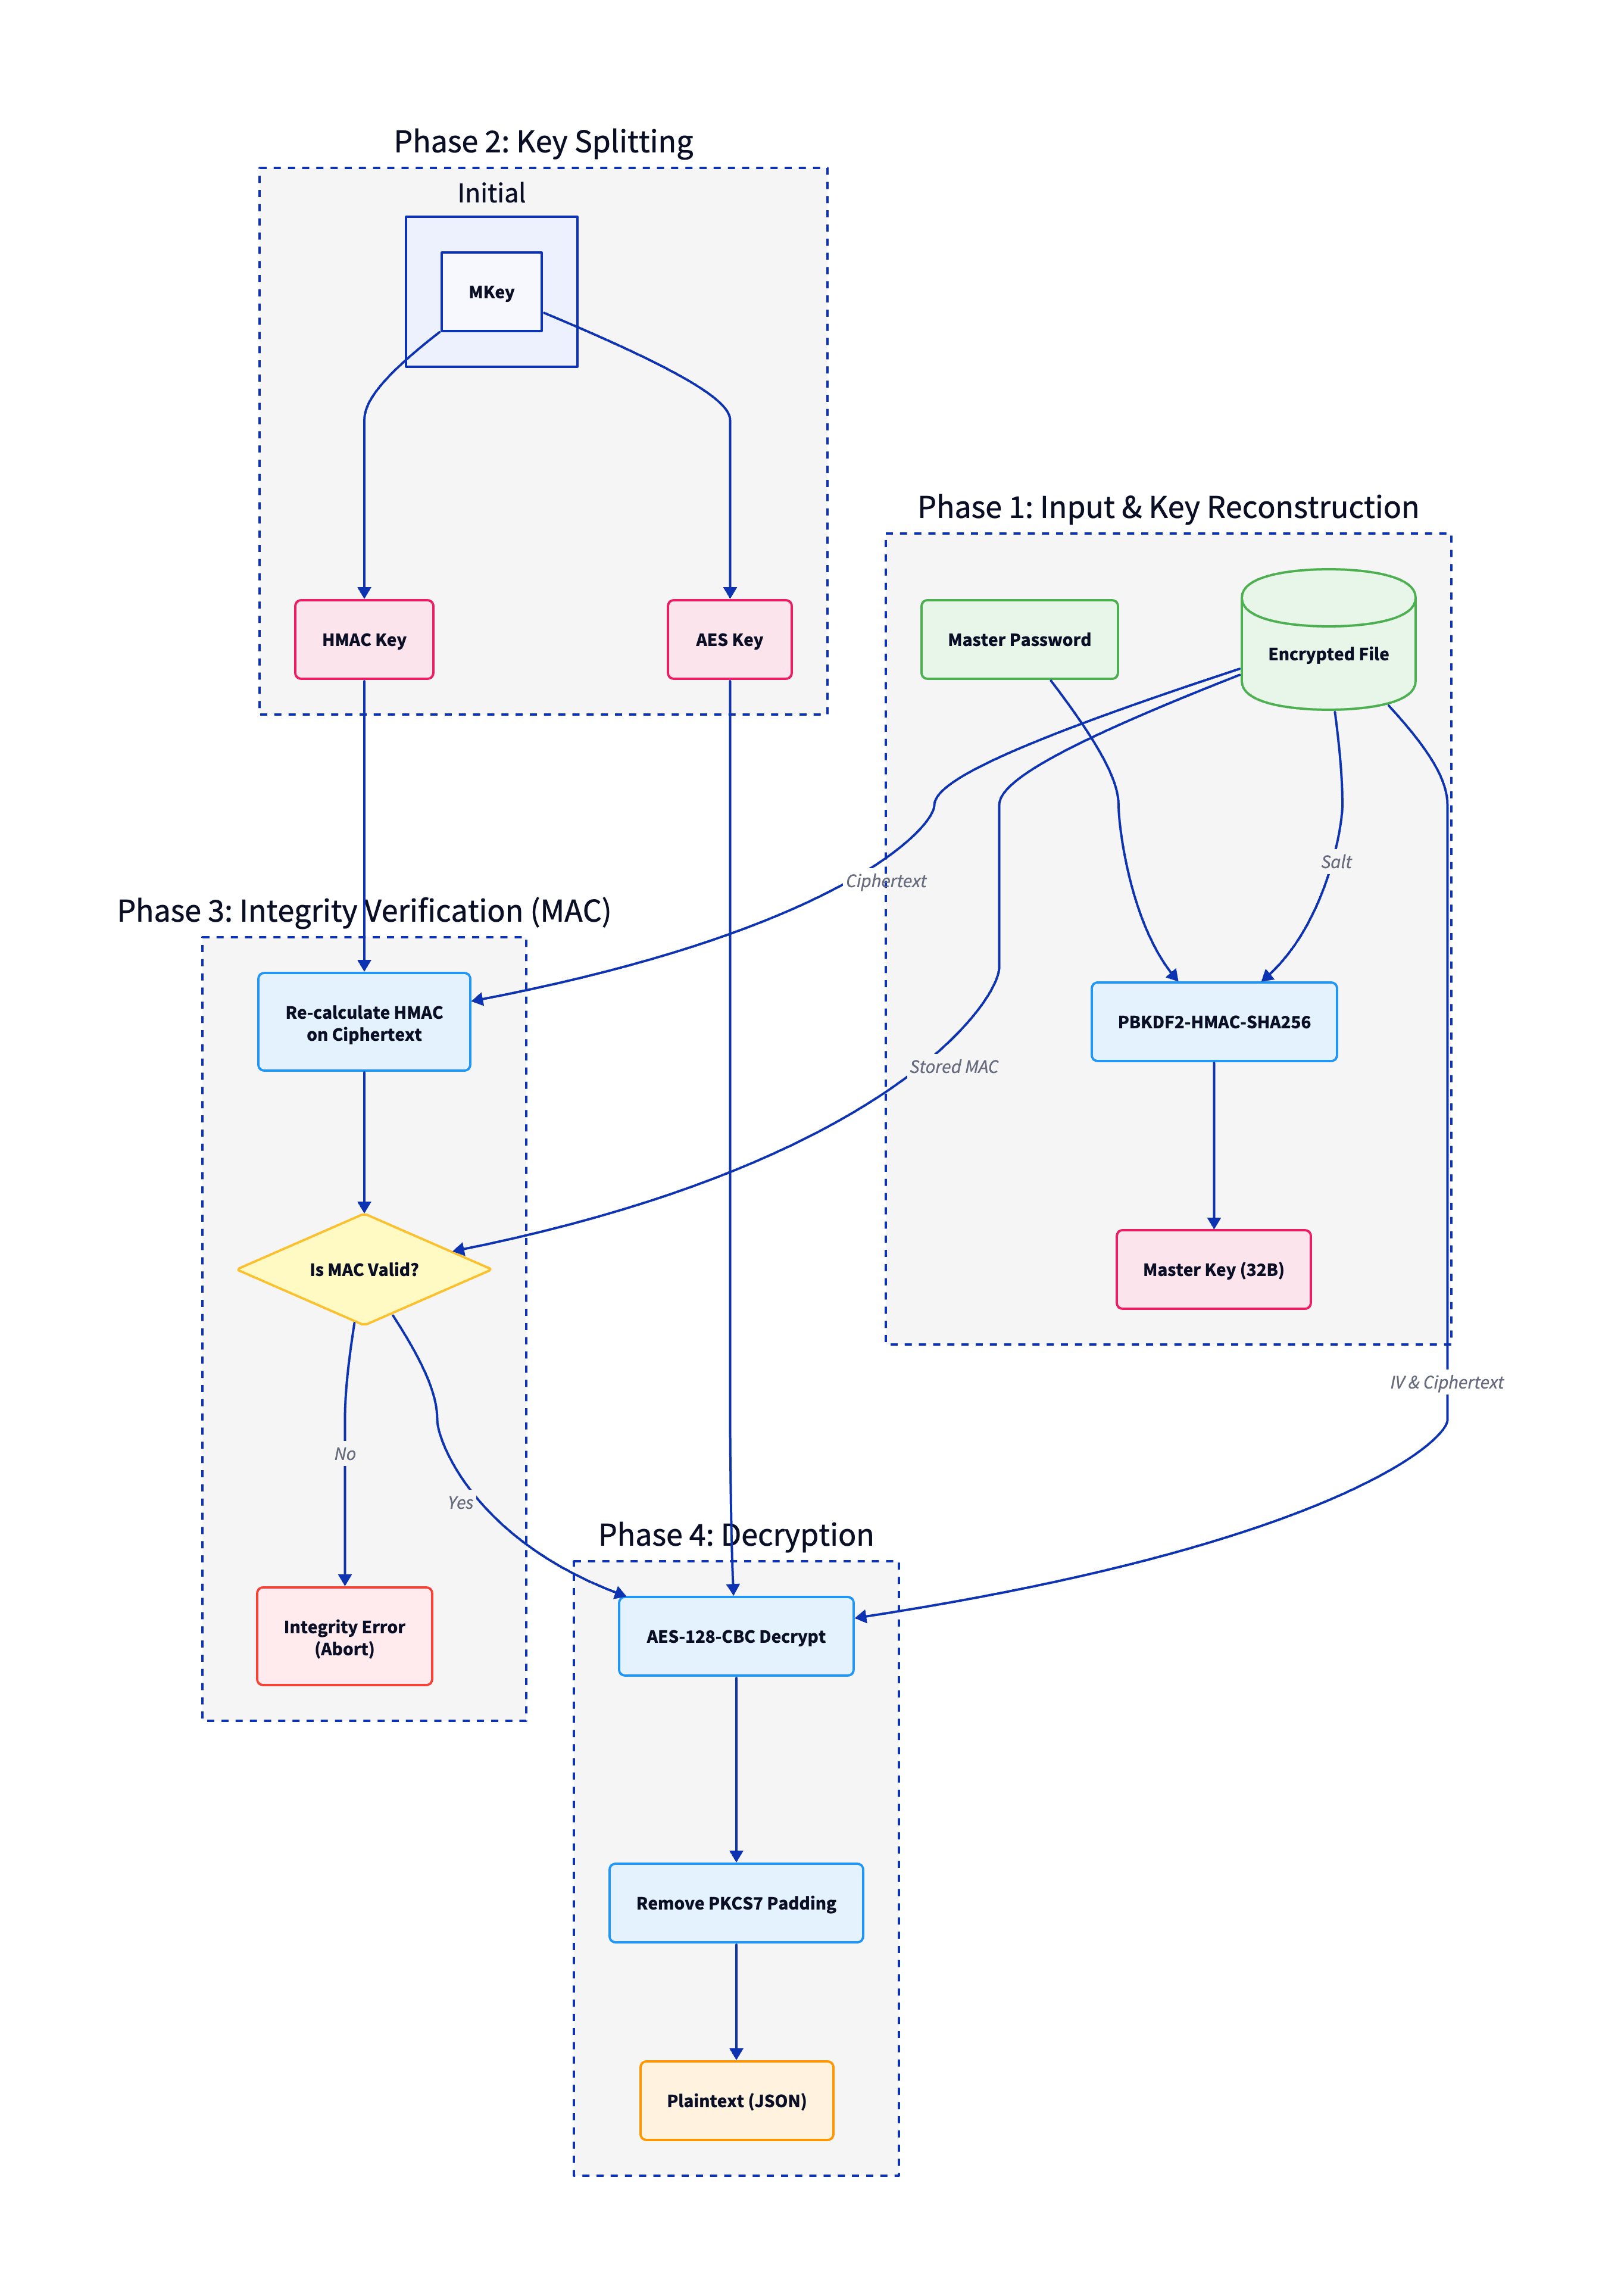
\includegraphics[width=0.8\textwidth]{../figure/figure_1b_decryption_flow.png}
    \caption{Phase-based Decryption Pipeline}
    \label{fig:dec_flow}
\end{figure}

\subsection{Design Justification: Cryptographic Key Splitting}
Following the derivation of a high-entropy Master Key ($MK$) via PBKDF2, a critical architectural decision is executed: \textbf{Key Splitting}. The 64-byte $MK$ is bisected to produce two mathematically independent 32-byte keys: an AES Key ($K_{enc}$) for confidentiality and an HMAC Key ($K_{mac}$) for integrity.

This separation of concerns is a fundamental requirement for secure system design. As formally analyzed by Bellare and Namprempre \cite{bellare2000}, deploying the \textit{same} cryptographic key for both the symmetric encryption scheme and the Message Authentication Code (MAC) inherently invalidates the generic security proofs of the composition. Reusing a key introduces perilous cross-primitive correlations, potentially allowing an adversary to leverage weaknesses or state from the MAC function to compromise the block cipher, or vice versa. By deriving $K_{enc}$ and $K_{mac}$ independently, the system guarantees that the confidentiality and integrity mechanisms remain cryptographically isolated and secure.

\subsection{Encryption Phase}
The encryption phase transforms the serialized vault data from plaintext into an opaque ciphertext through a series of deterministic transformations. Initially, the system utilizes a cryptographically secure pseudo-random number generator (CSPRNG) to produce a unique 16-byte Initialization Vector ($IV$), ensuring that identical plaintexts result in distinct ciphertexts over multiple encryption cycles. Before the cryptographic core is engaged, the plaintext payload is processed using the PKCS\#7 specification, adding defensive padding to align the data length with the 16-byte block size mandated by the cipher. Finally, the AES algorithm is executed in Cipher Block Chaining (CBC) mode, utilizing the dedicated encryption key and the generated $IV$ to yield the final ciphertext ($C$).

\subsection{Authentication Phase}
To achieve comprehensive security against chosen-ciphertext attacks, the system strictly implements the Encrypt-then-MAC (EtM) paradigm. Following the ciphertext production, a Message Authentication Code is generated to bind the encrypted data to its specific context. This is accomplished by concatenating the $IV$ with the ciphertext ($C$) to form a comprehensive authentication payload. The HMAC-SHA256 algorithm is then applied to this payload using the dedicated $K_{mac}$, producing a 32-byte authentication tag ($Tag$). This architecture ensures the integrity of the entire encrypted package, allowing the system to detect any unauthorized modifications to either the ciphertext or the $IV$ before the decryption logic is ever exercised.

\section{Vault Data Structure}

\subsection{Binary Layout Formatting}
The output of the cryptographic pipeline is serialized into a rigid binary format to ensure interoperability and parameter persistence as visualized in Figure \ref{fig:file_format}. This structure adheres to the security recommendations of NIST SP 800-132 regarding the adjacent storage of KDF parameters and protected data. 

\begin{figure}[H]
    \centering
    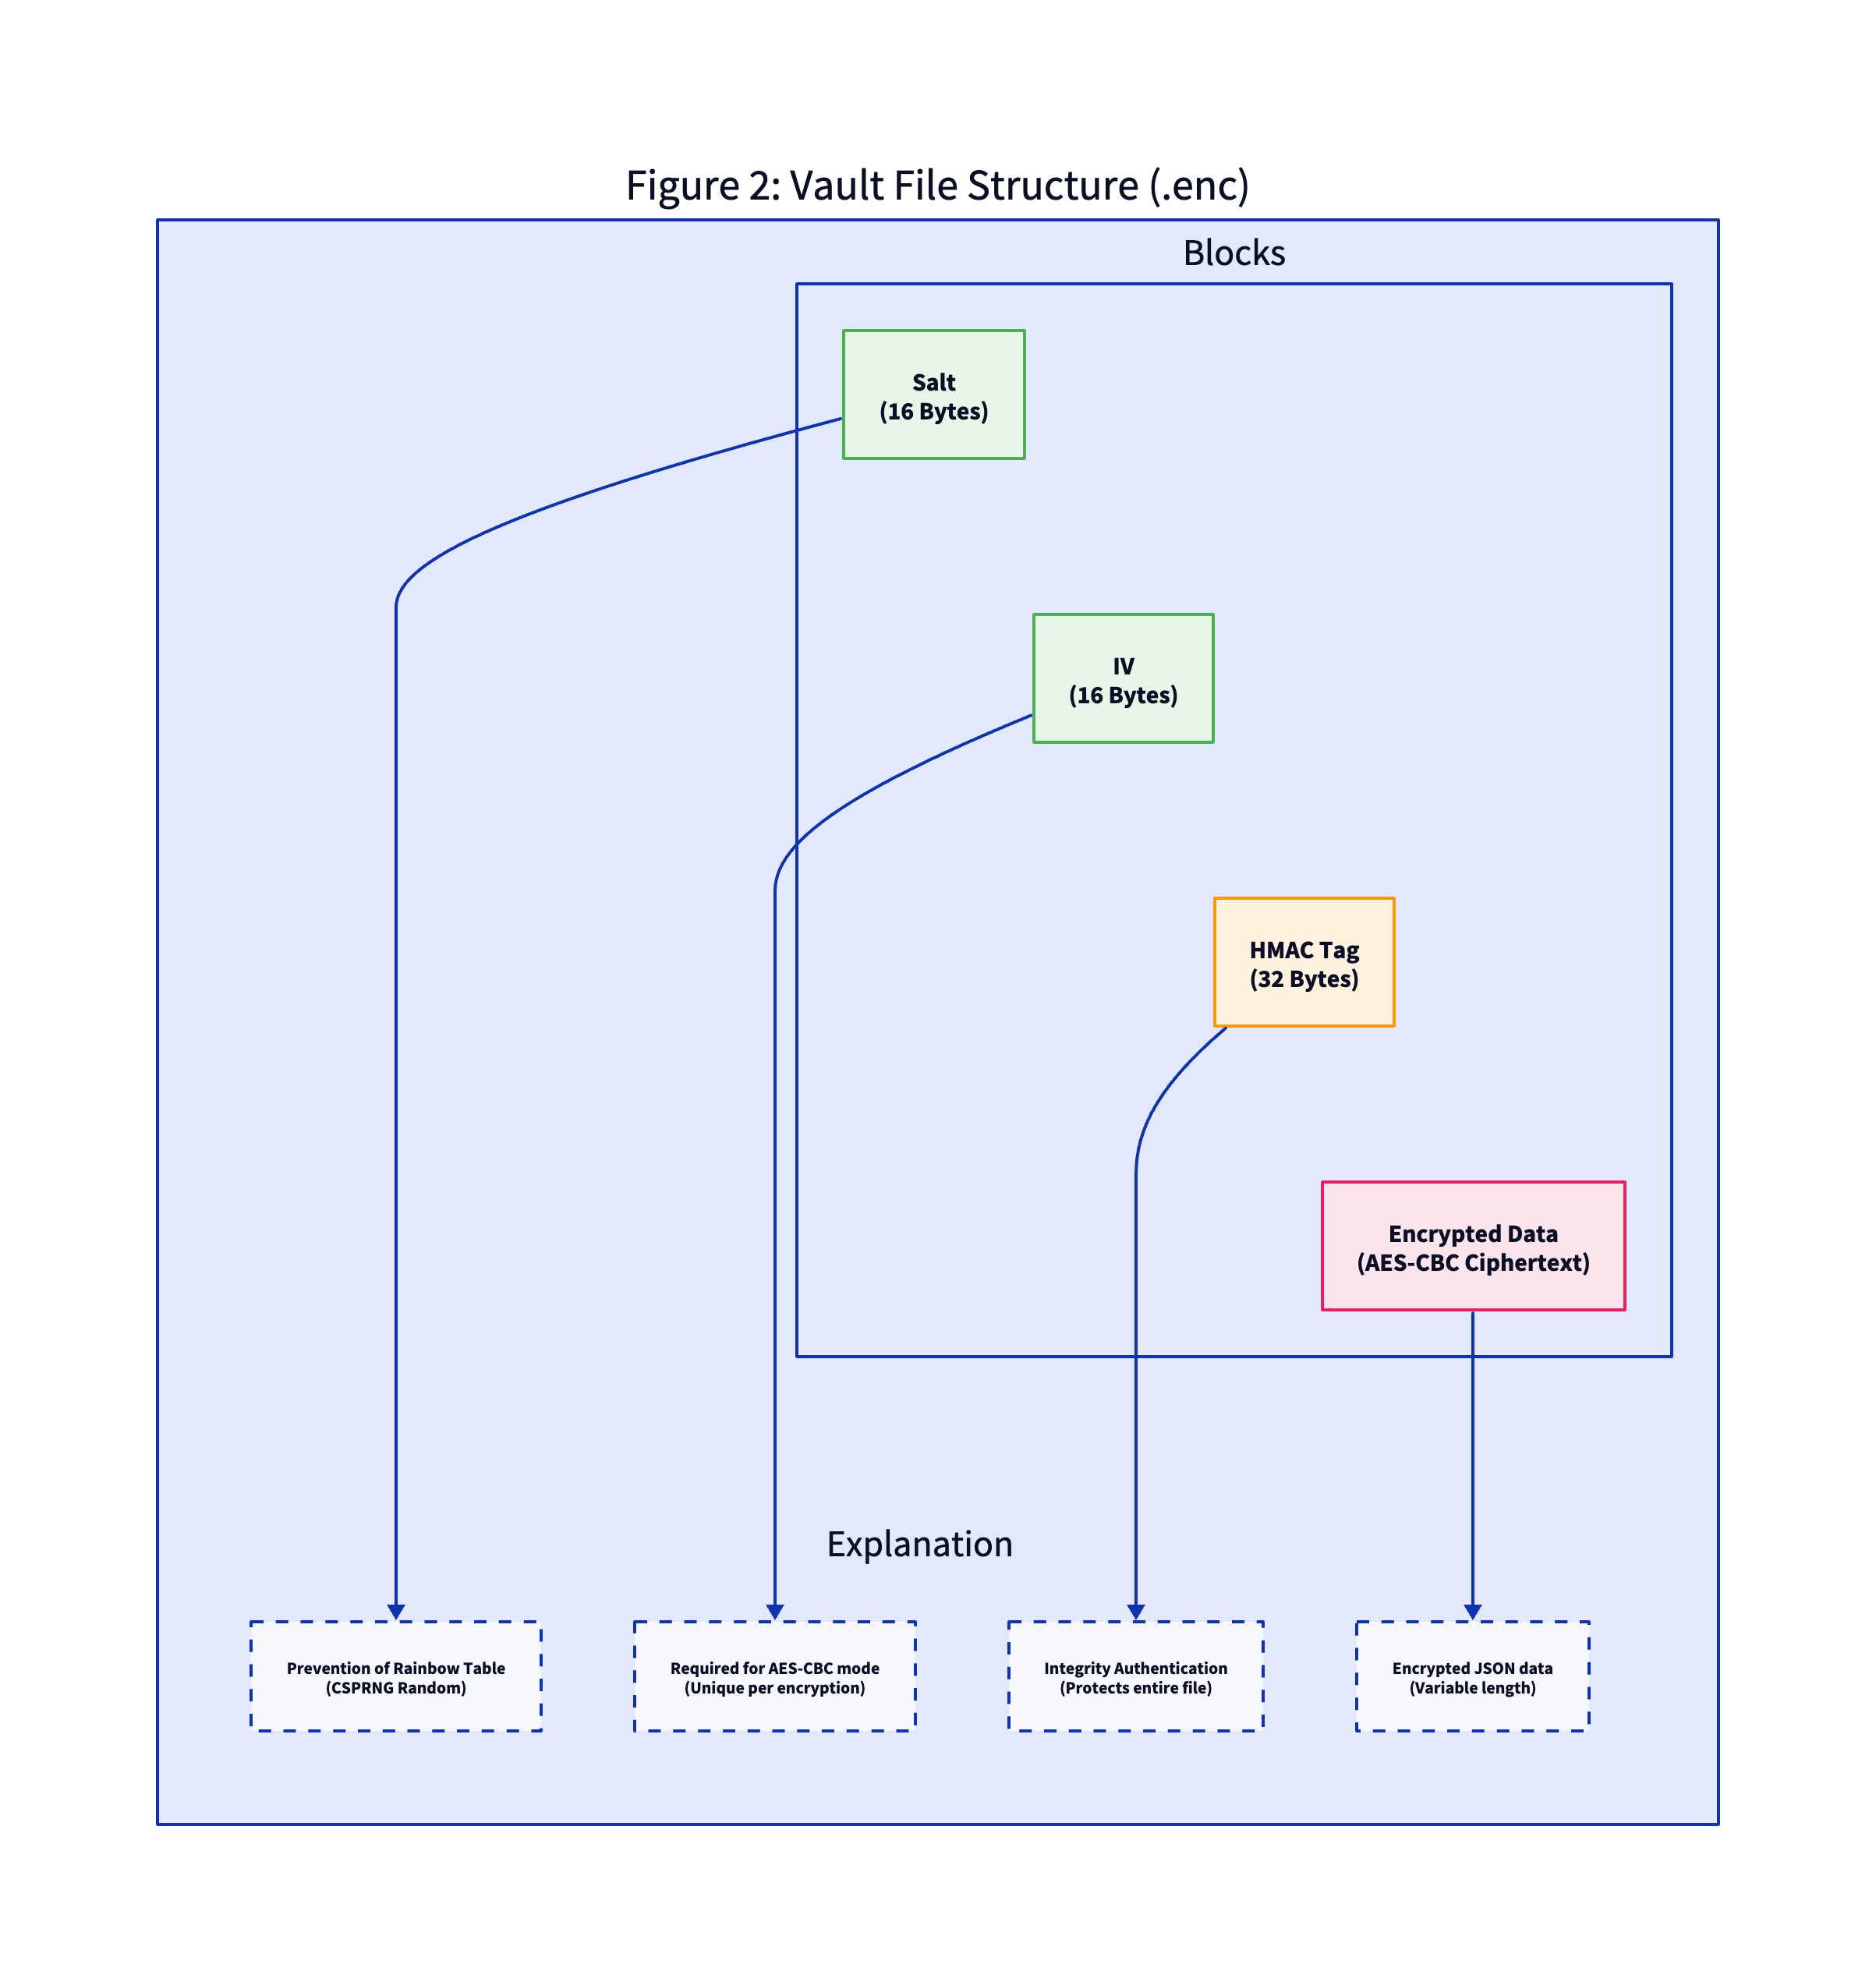
\includegraphics[width=0.8\textwidth]{../figure/figure_2_file_format.png}
    \caption{Binary Vault File Format}
    \label{fig:file_format}
\end{figure}

The vault file consists of four contiguous segments: a 16-byte random Salt for key derivation, a 16-byte $IV$ for the block cipher, and a 32-byte HMAC-SHA256 $Tag$ for integrity verification. These parameters precede the variable-length ciphertext, facilitating a linear parsing routine that can reconstruct the cryptographic state required for safe data retrieval.

\subsection{Safe Decryption and Verification Process}
The retrieval of plaintext data from the vault hinges upon the uncompromising principles of the EtM composition, which dictates that authentication must precede any decryption transformation. The process begins with the reconstruction of the Master Key ($MK$) using the retrieved Salt and the user's password, followed by a secondary key splitting to recover $K_{enc}$ and $K_{mac}$. Before the AES cipher is initialized, the system computes a candidate MAC from the stored $IV$ and ciphertext. 

A constant-time comparison is then performed between the candidate and the stored $Tag$. In the event of a verification failure, the system immediately rejects the vault as compromised, aborting the routine without ever invoking the AES decryption function. This critical invariant completely neutralizes potential vulnerabilities to padding oracle attacks. A constant-time comparison is then performed between the candidate and the stored $Tag$. In the event of a verification failure, the system immediately rejects the vault as compromised, aborting the routine without ever invoking the AES decryption function. This critical invariant completely neutralizes potential vulnerabilities to padding oracle attacks. Only upon a successful integrity match is the AES-128-CBC decryption initialized, transforming the ciphertext back into plaintext and stripping the PKCS\#7 padding to recover the original data.

\begin{lstlisting}[language=Python, caption=Safe Authentication and Decryption Flow, label=lst:decryption]
def decrypt_vault(ciphertext, iv, stored_mac, aes_key, hmac_key):
    # 1. Integrity Check: Verify HMAC BEFORE Decryption
    h = hmac.HMAC(hmac_key, hashes.SHA256())
    h.update(ciphertext)
    h.verify(stored_mac) # Throws error if mismatch

    # 2. Decryption: AES-128-CBC
    cipher = Cipher(algorithms.AES(aes_key), modes.CBC(iv))
    decryptor = cipher.decryptor()
    padded_data = decryptor.update(ciphertext) + decryptor.finalize()

    # 3. Remove PKCS7 Padding
    unpadder = padding.PKCS7(128).unpadder()
    return unpadder.update(padded_data) + unpadder.finalize()
\end{lstlisting}
